\documentclass[11pt]{article}
\usepackage[margin=30mm]{geometry}
\usepackage{tikz}
\usepackage{xcolor}
\usepackage{amsmath}
\usepackage{caption}
\usepackage{subcaption}
\usepackage{stmaryrd}
\usepackage{amssymb}
\usepackage{graphicx}
\pagestyle{empty}
\addtolength{\skip\footins}{10pt}

\title{Membership functions 3}

\begin{document}

\subsection{Two graded membership functions derived from a superposition of Voronoi diagrams}

\subsubsection*{Combinatorial membership function}
Let \(R=\{r_1,\dots,r_m\}\) be prototypical regions. For each \(i\) let \(P_i=\{p_{i1},\dots,p_{i,n_i}\}\subset\mathbb{R}^2\) be a finite set of candidate prototypes contained in \(r_i\). The set of all ordered configurations (one choice per region) is
\[
\Pi(R):=\prod_{i=1}^m P_i=\{\langle p_1,\dots,p_m\rangle \mid p_i\in P_i\},
\qquad N:=|\Pi(R)|= n^m.
\]
For \(\mathbf p\in\Pi(R)\) denote by \(V_i(\mathbf p)\) the Voronoi cell\footnote{$V(p_i) := \{p \mid \delta_S(p, p_i) \le \delta_S(p, p_j), \text{ for all } j \in \{1, \ldots, n\} \text{ with } j \ne i\}$} of the \(i\)-th prototype in the Voronoi diagram generated by \(\{p_1,\dots,p_m\}\). The combinatorial membership degree of \(x\in\mathbb{R}^2\) to the concept \(C_i\) (associated with \(r_i\)) can be written equivalently in the two forms below:
\[
M_{C_i}(x)
= \frac{1}{N}\sum_{\mathbf p\in\Pi(R)} \mathbf{1}\big(x\in V_i(\mathbf p)\big)
= \frac{\big|\{\mathbf p\in\Pi(R)\mid x\in V_i(\mathbf p)\}\big|}{|\Pi(R)|}.
\]

We can critique this combinatorial function.
First, the function \(M_{C_i}\) is a finite rational-valued step function: for every \(x\), \(M_{C_i}(x)\in\{0,\frac{1}{N},\dots,1\}\). It is piecewise constant (discontinuities occur exactly on the union of Voronoi boundaries across all configurations).

Human graded membership data are typically fit better by smooth curves than by step functions. The combinatorial form is simple and transparent but may produce implausible abrupt jumps when a point crosses an atomic cell boundary.

\subsubsection*{Continuous graded membership}
We can replace the finite prototype sets \(P_i\) by measurable prototypical areas \(r_i\subset\mathbb{R}^2\). The idea is to choose one prototype from each region \(r_i\) according to the Lebesgue measure and measure the proportion of choices that make a given point \(a\) fall in the cell of concept \(C_i\). This yields a continuous graded-membership function that generalizes the discrete counting proportion.
First, define the configuration (completion) space
\[
\Pi(R) := \prod_{i=1}^m r_i \subset (\mathbb{R}^2)^m,
\]
whose generic element we write as \(\mathbf p=(p_1,\dots,p_m)\) with \(p_i\in r_i\). We endow \(\Pi(R)\) with the product Lebesgue measure \(\mu\); thus
\[
\mu(\Pi(R)) = \prod_{i=1}^m \operatorname{vol}(r_i),
\]
which is finite when each prototypical area \(r_i\) is bounded.

Now, we can define the continuous membership function.
Fix \(a\in\mathbb{R}^2\) and an index \(i\). Let
\[
S_{a,i} := \{\mathbf p\in\Pi(R)\mid \delta(a,p_i) < \delta(a,p_j)\ \text{for all } j\neq i\},
\]
where \(\delta\) denotes Euclidean distance. The measure of \(S_{a,i}\) is
\[
\mu(S_{a,i})=\int_{\Pi(R)} \mathbf{1}_{S_{a,i}}(\mathbf p)\,d\mu(\mathbf p),
\]
and the continuous graded-membership degree is defined by
\[
M_{C_i}(a) \;:=\; \frac{\mu(S_{a,i})}{\mu(\Pi(R))}.
\]

\begin{figure}[!ht]
  \centering

  % Tabular with two fixed-width columns so the items stay on the same row
    \begin{tabular}{@{}p{6.000000cm}@{\hspace{0.600000cm}}p{6.000000cm}@{}}
    \centering
    \begin{subfigure}[t]{6.000000cm}
      \centering
      % Left tikz (scaled to fill width)
      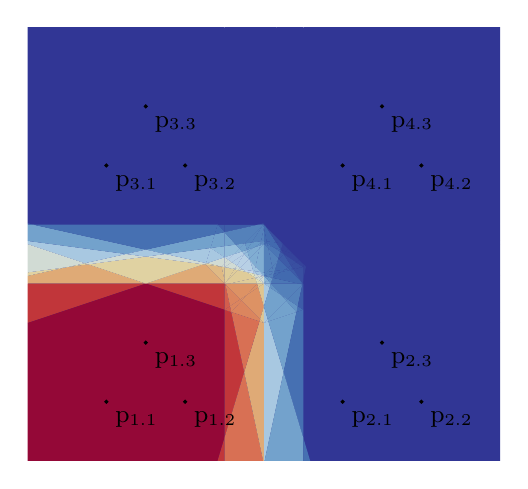
\begin{tikzpicture}[x=1.000000cm,y=1.000000cm]
        \useasboundingbox (-0.500000,-0.500000) rectangle (5.500000,5.000000);
        \clip (-0.500000,-0.500000) rectangle (5.500000,5.000000);
\useasboundingbox (-0.5,-0.5) rectangle (5.5,5.0);

\definecolor{bgcol}{rgb}{0.192157,0.211765,0.584314}
\definecolor{c1}{rgb}{0.875359,0.771895,0.561503}
\definecolor{c2}{rgb}{0.874444,0.726144,0.518497}
\definecolor{c3}{rgb}{0.876144,0.798693,0.598366}
\definecolor{c4}{rgb}{0.820065,0.859020,0.832353}
\definecolor{c5}{rgb}{0.588039,0.746471,0.859608}
\definecolor{c6}{rgb}{0.451438,0.637190,0.800000}
\definecolor{c7}{rgb}{0.239216,0.360000,0.657255}
\definecolor{c8}{rgb}{0.192157,0.211765,0.584314}
\definecolor{c9}{rgb}{0.852745,0.471569,0.346275}
\definecolor{c10}{rgb}{0.866863,0.573529,0.393333}
\definecolor{c11}{rgb}{0.878627,0.875686,0.715098}
\definecolor{c12}{rgb}{0.544902,0.711961,0.840784}
\definecolor{c13}{rgb}{0.329477,0.505948,0.731242}
\definecolor{c14}{rgb}{0.292614,0.462026,0.708497}
\definecolor{c15}{rgb}{0.257516,0.417647,0.685621}
\definecolor{c16}{rgb}{0.223529,0.310588,0.632941}
\definecolor{c17}{rgb}{0.873268,0.667320,0.463203}
\definecolor{c18}{rgb}{0.754967,0.211699,0.226797}
\definecolor{c19}{rgb}{0.876928,0.823007,0.635229}
\definecolor{c20}{rgb}{0.848039,0.437582,0.330588}
\definecolor{c21}{rgb}{0.826993,0.363203,0.296340}
\definecolor{c22}{rgb}{0.578824,0.031765,0.214314}
\definecolor{c23}{rgb}{0.848431,0.870000,0.780196}
\definecolor{c24}{rgb}{0.720065,0.814575,0.898627}
\definecolor{c25}{rgb}{0.501765,0.677451,0.821961}
\definecolor{c26}{rgb}{0.207843,0.261176,0.608627}
\definecolor{c27}{rgb}{0.274183,0.440065,0.697124}
\definecolor{c28}{rgb}{0.372484,0.557190,0.757778}
\definecolor{c29}{rgb}{0.215686,0.285882,0.620784}
\definecolor{c30}{rgb}{0.859804,0.522549,0.369804}
\definecolor{c31}{rgb}{0.657712,0.783987,0.880980}
\definecolor{c32}{rgb}{0.523333,0.694706,0.831373}
\definecolor{c33}{rgb}{0.409346,0.601111,0.780523}
\definecolor{c34}{rgb}{0.390915,0.579150,0.769150}
\definecolor{c35}{rgb}{0.832222,0.863725,0.810000}
\definecolor{c36}{rgb}{0.678497,0.794183,0.886863}
\definecolor{c37}{rgb}{0.636928,0.773791,0.875098}
\definecolor{c38}{rgb}{0.768562,0.838366,0.912353}
\filldraw[draw=none,fill=bgcol] (-0.5,-0.5) rectangle (5.5,5.0);
\begin{scope}\clip (-0.5,-0.5) rectangle (5.5,5.0);

\filldraw[draw=none,fill=c1] (2.0,1.75) -- (2.0,1.791667) -- (2.007353,1.757353) -- (2.0,1.75) -- cycle;
\filldraw[draw=none,fill=c2] (2.0,1.791667) -- (2.0,1.75) -- (1.759615,1.990385) -- (1.963235,1.963235) -- (2.0,1.791667) -- cycle;
\filldraw[draw=none,fill=c3] (2.0,1.791667) -- (2.0,1.958333) -- (2.125,1.930556) -- (2.025,1.775) -- (2.007353,1.757353) -- (2.0,1.791667) -- cycle;
\filldraw[draw=none,fill=c1] (2.0,1.958333) -- (2.0,1.791667) -- (1.963235,1.963235) -- (2.0,1.958333) -- cycle;
\filldraw[draw=none,fill=c4] (2.0,1.958333) -- (2.0,2.0) -- (2.05,2.05) -- (2.09375,2.020833) -- (2.0,1.958333) -- cycle;
\filldraw[draw=none,fill=c4] (2.0,2.0) -- (2.0,1.958333) -- (1.965909,1.965909) -- (2.0,2.0) -- cycle;
\filldraw[draw=none,fill=c4] (2.0,2.0) -- (2.0,2.083333) -- (2.05,2.05) -- (2.0,2.0) -- cycle;
\filldraw[draw=none,fill=c4] (2.0,2.083333) -- (2.0,2.0) -- (1.965909,1.965909) -- (1.775,2.008333) -- (2.0,2.083333) -- cycle;
\filldraw[draw=none,fill=c5] (2.0,2.083333) -- (2.0,2.225) -- (2.142857,2.244048) -- (2.190789,2.190789) -- (2.125,2.125) -- (2.0,2.083333) -- cycle;
\filldraw[draw=none,fill=c5] (2.0,2.225) -- (2.0,2.083333) -- (1.822917,2.201389) -- (2.0,2.225) -- cycle;
\filldraw[draw=none,fill=c6] (2.0,2.225) -- (2.0,2.402778) -- (2.142857,2.244048) -- (2.0,2.225) -- cycle;
\filldraw[draw=none,fill=c6] (2.0,2.402778) -- (2.0,2.225) -- (1.822917,2.201389) -- (1.875,2.375) -- (2.0,2.402778) -- cycle;
\filldraw[draw=none,fill=c7] (2.0,2.402778) -- (2.0,2.5) -- (2.4375,2.5) -- (2.0,2.402778) -- cycle;
\filldraw[draw=none,fill=c7] (2.0,2.5) -- (2.0,2.402778) -- (1.9125,2.5) -- (2.0,2.5) -- cycle;
\filldraw[draw=none,fill=c8] (2.0,2.5) -- (2.0,2.791667) -- (2.25,3.625) -- (2.488636,2.511364) -- (2.4375,2.5) -- (2.0,2.5) -- cycle;
\filldraw[draw=none,fill=c8] (2.0,2.791667) -- (2.0,2.5) -- (1.9125,2.5) -- (2.0,2.791667) -- cycle;
\filldraw[draw=none,fill=c8] (2.0,2.791667) -- (2.0,4.791667) -- (2.25,3.625) -- (2.0,2.791667) -- cycle;
\filldraw[draw=none,fill=c8] (2.0,4.791667) -- (2.0,2.791667) -- (1.9125,2.5) -- (-0.4375,2.5) -- (-1.0,2.625) -- (-1.0,11.0) -- (0.5375,11.0) -- (1.0,9.458333) -- (2.0,4.791667) -- cycle;
\filldraw[draw=none,fill=c8] (2.0,4.791667) -- (2.0,6.125) -- (2.5,4.458333) -- (2.25,3.625) -- (2.0,4.791667) -- cycle;
\filldraw[draw=none,fill=c8] (2.0,6.125) -- (2.0,4.791667) -- (1.0,9.458333) -- (2.0,6.125) -- cycle;
\filldraw[draw=none,fill=c8] (2.0,6.125) -- (2.0,11.0) -- (2.5,11.0) -- (2.5,4.458333) -- (2.0,6.125) -- cycle;
\filldraw[draw=none,fill=c8] (2.0,11.0) -- (2.0,6.125) -- (1.0,9.458333) -- (0.669643,11.0) -- (2.0,11.0) -- cycle;
\filldraw[draw=none,fill=c9] (2.0,1.75) -- (2.008929,1.75) -- (2.011364,1.738636) -- (2.0,1.75) -- cycle;
\filldraw[draw=none,fill=c1] (2.008929,1.75) -- (2.0,1.75) -- (2.007353,1.757353) -- (2.008929,1.75) -- cycle;
\filldraw[draw=none,fill=c10] (2.008929,1.75) -- (2.0625,1.75) -- (2.011364,1.738636) -- (2.008929,1.75) -- cycle;
\filldraw[draw=none,fill=c3] (2.0625,1.75) -- (2.008929,1.75) -- (2.025,1.775) -- (2.170455,1.920455) -- (2.28125,1.895833) -- (2.292994,1.888004) -- (2.381387,1.829075) -- (2.390625,1.822917) -- (2.0625,1.75) -- cycle;
\filldraw[draw=none,fill=c10] (2.0625,1.75) -- (2.4125,1.75) -- (2.28125,1.604167) -- (2.2,1.55) -- (2.011364,1.738636) -- (2.0625,1.75) -- cycle;
\filldraw[draw=none,fill=c3] (2.4125,1.75) -- (2.0625,1.75) -- (2.390625,1.822917) -- (2.4125,1.75) -- cycle;
\filldraw[draw=none,fill=c1] (2.4125,1.75) -- (2.5,1.75) -- (2.427083,1.701389) -- (2.4125,1.75) -- cycle;
\filldraw[draw=none,fill=c11] (2.5,1.75) -- (2.4125,1.75) -- (2.420192,1.758547) -- (2.445312,1.786458) -- (2.5,1.75) -- cycle;
\filldraw[draw=none,fill=c5] (2.5,1.75) -- (2.5875,1.75) -- (2.572917,1.701389) -- (2.5,1.75) -- cycle;
\filldraw[draw=none,fill=c12] (2.5875,1.75) -- (2.5,1.75) -- (2.554688,1.786458) -- (2.579808,1.758547) -- (2.5875,1.75) -- cycle;
\filldraw[draw=none,fill=c13] (2.5875,1.75) -- (2.9375,1.75) -- (2.988636,1.738636) -- (2.8,1.55) -- (2.71875,1.604167) -- (2.5875,1.75) -- cycle;
\filldraw[draw=none,fill=c14] (2.9375,1.75) -- (2.5875,1.75) -- (2.609375,1.822917) -- (2.9375,1.75) -- cycle;
\filldraw[draw=none,fill=c14] (2.9375,1.75) -- (2.991071,1.75) -- (2.988636,1.738636) -- (2.9375,1.75) -- cycle;
\filldraw[draw=none,fill=c15] (2.991071,1.75) -- (2.9375,1.75) -- (2.609375,1.822917) -- (2.652344,1.851562) -- (2.71875,1.895833) -- (2.829545,1.920455) -- (2.975,1.775) -- (2.991071,1.75) -- cycle;
\filldraw[draw=none,fill=c7] (2.991071,1.75) -- (3.0,1.75) -- (2.988636,1.738636) -- (2.991071,1.75) -- cycle;
\filldraw[draw=none,fill=c16] (3.0,1.75) -- (2.991071,1.75) -- (2.992647,1.757353) -- (3.0,1.75) -- cycle;
\filldraw[draw=none,fill=c8] (3.0,1.75) -- (4.0,1.75) -- (3.0,1.416667) -- (3.0,1.75) -- cycle;
\filldraw[draw=none,fill=c8] (4.0,1.75) -- (3.0,1.75) -- (3.240385,1.990385) -- (3.267857,1.994048) -- (4.0,1.75) -- cycle;
\filldraw[draw=none,fill=c8] (4.0,1.75) -- (5.9375,1.75) -- (11.0,0.625) -- (11.0,-0.583333) -- (4.0,1.75) -- cycle;
\filldraw[draw=none,fill=c8] (5.9375,1.75) -- (4.0,1.75) -- (4.732143,1.994048) -- (5.0,1.958333) -- (5.9375,1.75) -- cycle;
\filldraw[draw=none,fill=c8] (5.9375,1.75) -- (6.5625,1.75) -- (11.0,1.158333) -- (11.0,0.625) -- (5.9375,1.75) -- cycle;
\filldraw[draw=none,fill=c8] (6.5625,1.75) -- (5.9375,1.75) -- (5.0,1.958333) -- (6.5625,1.75) -- cycle;
\filldraw[draw=none,fill=c8] (6.5625,1.75) -- (11.0,1.75) -- (11.0,1.158333) -- (6.5625,1.75) -- cycle;
\filldraw[draw=none,fill=c8] (11.0,1.75) -- (6.5625,1.75) -- (5.0,1.958333) -- (4.775,2.008333) -- (5.708333,2.319444) -- (7.0625,2.5) -- (11.0,2.5) -- (11.0,1.75) -- cycle;
\filldraw[draw=none,fill=c17] (2.0,1.75) -- (1.0,1.75) -- (1.732143,1.994048) -- (1.759615,1.990385) -- (2.0,1.75) -- cycle;
\filldraw[draw=none,fill=c18] (1.0,1.75) -- (2.0,1.75) -- (2.0,1.416667) -- (1.0,1.75) -- cycle;
\filldraw[draw=none,fill=c17] (1.0,1.75) -- (-0.9375,1.75) -- (-0.0,1.958333) -- (0.267857,1.994048) -- (1.0,1.75) -- cycle;
\filldraw[draw=none,fill=c18] (-0.9375,1.75) -- (1.0,1.75) -- (-1.0,1.083333) -- (-1.0,1.736111) -- (-0.9375,1.75) -- cycle;
\filldraw[draw=none,fill=c19] (-0.9375,1.75) -- (-1.0,1.75) -- (-1.0,1.825) -- (-0.0,1.958333) -- (-0.9375,1.75) -- cycle;
\filldraw[draw=none,fill=c20] (-1.0,1.75) -- (-0.9375,1.75) -- (-1.0,1.736111) -- (-1.0,1.75) -- cycle;
\filldraw[draw=none,fill=c21] (2.0,1.416667) -- (2.0,1.75) -- (2.011364,1.738636) -- (2.070312,1.463542) -- (2.0,1.416667) -- cycle;
\filldraw[draw=none,fill=c22] (2.0,1.416667) -- (2.0,-0.208333) -- (1.7625,-1.0) -- (-1.0,-1.0) -- (-1.0,1.083333) -- (1.0,1.75) -- (2.0,1.416667) -- cycle;
\filldraw[draw=none,fill=c18] (2.0,-0.208333) -- (2.0,1.416667) -- (2.086538,1.387821) -- (2.25,0.625) -- (2.0,-0.208333) -- cycle;
\filldraw[draw=none,fill=c18] (2.0,-0.208333) -- (2.0,-1.0) -- (1.7625,-1.0) -- (2.0,-0.208333) -- cycle;
\filldraw[draw=none,fill=c20] (2.0,-1.0) -- (2.0,-0.208333) -- (2.25,0.625) -- (2.5,-0.541667) -- (2.401786,-1.0) -- (2.0,-1.0) -- cycle;
\filldraw[draw=none,fill=c3] (2.007353,1.757353) -- (2.025,1.775) -- (2.008929,1.75) -- (2.007353,1.757353) -- cycle;
\filldraw[draw=none,fill=c3] (2.170455,1.920455) -- (2.025,1.775) -- (2.125,1.930556) -- (2.170455,1.920455) -- cycle;
\filldraw[draw=none,fill=c23] (2.170455,1.920455) -- (2.183824,1.933824) -- (2.234375,1.927083) -- (2.28125,1.895833) -- (2.170455,1.920455) -- cycle;
\filldraw[draw=none,fill=c23] (2.183824,1.933824) -- (2.170455,1.920455) -- (2.125,1.930556) -- (2.131579,1.940789) -- (2.183824,1.933824) -- cycle;
\filldraw[draw=none,fill=c4] (2.183824,1.933824) -- (2.2,1.95) -- (2.234375,1.927083) -- (2.183824,1.933824) -- cycle;
\filldraw[draw=none,fill=c4] (2.2,1.95) -- (2.183824,1.933824) -- (2.131579,1.940789) -- (2.15625,1.979167) -- (2.2,1.95) -- cycle;
\filldraw[draw=none,fill=c24] (2.2,1.95) -- (2.309211,2.059211) -- (2.325,2.041667) -- (2.364583,1.909722) -- (2.234375,1.927083) -- (2.2,1.95) -- cycle;
\filldraw[draw=none,fill=c24] (2.309211,2.059211) -- (2.2,1.95) -- (2.15625,1.979167) -- (2.25,2.125) -- (2.309211,2.059211) -- cycle;
\filldraw[draw=none,fill=c5] (2.309211,2.059211) -- (2.317308,2.067308) -- (2.325,2.041667) -- (2.309211,2.059211) -- cycle;
\filldraw[draw=none,fill=c5] (2.317308,2.067308) -- (2.309211,2.059211) -- (2.25,2.125) -- (2.291667,2.152778) -- (2.317308,2.067308) -- cycle;
\filldraw[draw=none,fill=c25] (2.317308,2.067308) -- (2.443182,2.193182) -- (2.394231,1.964744) -- (2.325,2.041667) -- (2.317308,2.067308) -- cycle;
\filldraw[draw=none,fill=c25] (2.443182,2.193182) -- (2.317308,2.067308) -- (2.291667,2.152778) -- (2.375,2.208333) -- (2.451923,2.233974) -- (2.443182,2.193182) -- cycle;
\filldraw[draw=none,fill=c25] (2.443182,2.193182) -- (2.5,2.25) -- (2.5,1.891667) -- (2.454545,1.897727) -- (2.394231,1.964744) -- (2.443182,2.193182) -- cycle;
\filldraw[draw=none,fill=c25] (2.5,2.25) -- (2.443182,2.193182) -- (2.451923,2.233974) -- (2.5,2.25) -- cycle;
\filldraw[draw=none,fill=c14] (2.5,2.25) -- (2.548077,2.233974) -- (2.556818,2.193182) -- (2.5,2.25) -- cycle;
\filldraw[draw=none,fill=c14] (2.548077,2.233974) -- (2.5,2.25) -- (2.541667,2.263889) -- (2.548077,2.233974) -- cycle;
\filldraw[draw=none,fill=c14] (2.548077,2.233974) -- (2.625,2.208333) -- (2.708333,2.152778) -- (2.682692,2.067308) -- (2.556818,2.193182) -- (2.548077,2.233974) -- cycle;
\filldraw[draw=none,fill=c14] (2.625,2.208333) -- (2.548077,2.233974) -- (2.541667,2.263889) -- (2.625,2.208333) -- cycle;
\filldraw[draw=none,fill=c15] (2.625,2.208333) -- (2.715909,2.17803) -- (2.708333,2.152778) -- (2.625,2.208333) -- cycle;
\filldraw[draw=none,fill=c15] (2.715909,2.17803) -- (2.625,2.208333) -- (2.541667,2.263889) -- (2.536765,2.286765) -- (2.65625,2.270833) -- (2.715909,2.17803) -- cycle;
\filldraw[draw=none,fill=c26] (2.715909,2.17803) -- (2.778846,2.157051) -- (2.75,2.125) -- (2.715909,2.17803) -- cycle;
\filldraw[draw=none,fill=c26] (2.778846,2.157051) -- (2.715909,2.17803) -- (2.740385,2.259615) -- (2.809211,2.190789) -- (2.778846,2.157051) -- cycle;
\filldraw[draw=none,fill=c26] (2.778846,2.157051) -- (2.875,2.125) -- (2.95,2.05) -- (2.90625,2.020833) -- (2.75,2.125) -- (2.751647,2.12683) -- (2.778846,2.157051) -- cycle;
\filldraw[draw=none,fill=c26] (2.875,2.125) -- (2.778846,2.157051) -- (2.809211,2.190789) -- (2.875,2.125) -- cycle;
\filldraw[draw=none,fill=c8] (2.875,2.125) -- (3.0,2.083333) -- (2.95,2.05) -- (2.875,2.125) -- cycle;
\filldraw[draw=none,fill=c8] (3.0,2.083333) -- (2.875,2.125) -- (2.809211,2.190789) -- (2.857143,2.244048) -- (3.0,2.225) -- (3.0,2.083333) -- cycle;
\filldraw[draw=none,fill=c8] (3.0,2.083333) -- (3.225,2.008333) -- (3.034091,1.965909) -- (3.0,2.0) -- (3.0,2.083333) -- cycle;
\filldraw[draw=none,fill=c8] (3.225,2.008333) -- (3.0,2.083333) -- (3.177083,2.201389) -- (3.234375,2.010417) -- (3.225,2.008333) -- cycle;
\filldraw[draw=none,fill=c8] (3.225,2.008333) -- (3.236111,2.00463) -- (3.240385,1.990385) -- (3.036765,1.963235) -- (3.034091,1.965909) -- (3.225,2.008333) -- cycle;
\filldraw[draw=none,fill=c8] (3.236111,2.00463) -- (3.225,2.008333) -- (3.234375,2.010417) -- (3.236111,2.00463) -- cycle;
\filldraw[draw=none,fill=c8] (3.236111,2.00463) -- (3.267857,1.994048) -- (3.240385,1.990385) -- (3.236111,2.00463) -- cycle;
\filldraw[draw=none,fill=c8] (3.267857,1.994048) -- (3.236111,2.00463) -- (3.234375,2.010417) -- (3.75,2.125) -- (4.0,2.091667) -- (3.267857,1.994048) -- cycle;
\filldraw[draw=none,fill=c8] (4.0,1.75) -- (3.267857,1.994048) -- (4.0,2.091667) -- (4.732143,1.994048) -- (4.0,1.75) -- cycle;
\filldraw[draw=none,fill=c8] (4.0,1.75) -- (11.0,-0.583333) -- (11.0,-1.0) -- (3.2375,-1.0) -- (3.0,-0.208333) -- (3.0,1.416667) -- (4.0,1.75) -- cycle;
\filldraw[draw=none,fill=c27] (2.5,2.25) -- (2.5,2.291667) -- (2.525,2.275) -- (2.5,2.25) -- cycle;
\filldraw[draw=none,fill=c28] (2.5,2.291667) -- (2.5,2.25) -- (2.475,2.275) -- (2.5,2.291667) -- cycle;
\filldraw[draw=none,fill=c15] (2.5,2.291667) -- (2.5,2.458333) -- (2.536765,2.286765) -- (2.5,2.291667) -- cycle;
\filldraw[draw=none,fill=c13] (2.5,2.458333) -- (2.5,2.291667) -- (2.463235,2.286765) -- (2.5,2.458333) -- cycle;
\filldraw[draw=none,fill=c15] (2.5,2.458333) -- (2.5,2.5) -- (2.507353,2.492647) -- (2.5,2.458333) -- cycle;
\filldraw[draw=none,fill=c13] (2.5,2.5) -- (2.5,2.458333) -- (2.492647,2.492647) -- (2.5,2.5) -- cycle;
\filldraw[draw=none,fill=c26] (2.5,2.5) -- (2.5,2.513889) -- (2.505435,2.505435) -- (2.5,2.5) -- cycle;
\filldraw[draw=none,fill=c29] (2.5,2.513889) -- (2.5,2.5) -- (2.494565,2.505435) -- (2.5,2.513889) -- cycle;
\filldraw[draw=none,fill=c8] (2.5,2.513889) -- (2.5,4.458333) -- (2.75,3.625) -- (2.511364,2.511364) -- (2.5,2.513889) -- cycle;
\filldraw[draw=none,fill=c8] (2.5,4.458333) -- (2.5,2.513889) -- (2.488636,2.511364) -- (2.25,3.625) -- (2.5,4.458333) -- cycle;
\filldraw[draw=none,fill=c8] (2.5,4.458333) -- (2.5,11.0) -- (3.0,11.0) -- (3.0,6.125) -- (2.5,4.458333) -- cycle;
\filldraw[draw=none,fill=c27] (2.5,2.25) -- (2.525,2.275) -- (2.541667,2.263889) -- (2.5,2.25) -- cycle;
\filldraw[draw=none,fill=c15] (2.525,2.275) -- (2.536765,2.286765) -- (2.541667,2.263889) -- (2.525,2.275) -- cycle;
\filldraw[draw=none,fill=c15] (2.536765,2.286765) -- (2.525,2.275) -- (2.5,2.291667) -- (2.536765,2.286765) -- cycle;
\filldraw[draw=none,fill=c15] (2.536765,2.286765) -- (2.5,2.458333) -- (2.507353,2.492647) -- (2.525,2.475) -- (2.65625,2.270833) -- (2.536765,2.286765) -- cycle;
\filldraw[draw=none,fill=c13] (2.492647,2.492647) -- (2.5,2.458333) -- (2.463235,2.286765) -- (2.34375,2.270833) -- (2.475,2.475) -- (2.492647,2.492647) -- cycle;
\filldraw[draw=none,fill=c13] (2.492647,2.492647) -- (2.491071,2.5) -- (2.5,2.5) -- (2.492647,2.492647) -- cycle;
\filldraw[draw=none,fill=c13] (2.491071,2.5) -- (2.492647,2.492647) -- (2.475,2.475) -- (2.491071,2.5) -- cycle;
\filldraw[draw=none,fill=c7] (2.491071,2.5) -- (2.488636,2.511364) -- (2.494565,2.505435) -- (2.491071,2.5) -- cycle;
\filldraw[draw=none,fill=c7] (2.488636,2.511364) -- (2.491071,2.5) -- (2.4375,2.5) -- (2.488636,2.511364) -- cycle;
\filldraw[draw=none,fill=c8] (0.669643,11.0) -- (1.0,9.458333) -- (0.5375,11.0) -- (0.669643,11.0) -- cycle;
\filldraw[draw=none,fill=c16] (2.65625,2.270833) -- (2.740385,2.259615) -- (2.715909,2.17803) -- (2.65625,2.270833) -- cycle;
\filldraw[draw=none,fill=c16] (2.740385,2.259615) -- (2.65625,2.270833) -- (2.611213,2.34089) -- (2.525,2.475) -- (2.740385,2.259615) -- cycle;
\filldraw[draw=none,fill=c8] (2.740385,2.259615) -- (2.857143,2.244048) -- (2.809211,2.190789) -- (2.740385,2.259615) -- cycle;
\filldraw[draw=none,fill=c8] (2.857143,2.244048) -- (2.740385,2.259615) -- (2.525,2.475) -- (2.508929,2.5) -- (2.5625,2.5) -- (3.0,2.402778) -- (2.857143,2.244048) -- cycle;
\filldraw[draw=none,fill=c8] (3.0,2.225) -- (2.857143,2.244048) -- (3.0,2.402778) -- (3.0,2.225) -- cycle;
\filldraw[draw=none,fill=c8] (3.0,2.225) -- (3.177083,2.201389) -- (3.0,2.083333) -- (3.0,2.225) -- cycle;
\filldraw[draw=none,fill=c8] (3.177083,2.201389) -- (3.0,2.225) -- (3.0,2.402778) -- (3.125,2.375) -- (3.177083,2.201389) -- cycle;
\filldraw[draw=none,fill=c8] (3.177083,2.201389) -- (3.75,2.125) -- (3.234375,2.010417) -- (3.177083,2.201389) -- cycle;
\filldraw[draw=none,fill=c8] (3.75,2.125) -- (3.177083,2.201389) -- (3.125,2.375) -- (4.0,2.180556) -- (3.75,2.125) -- cycle;
\filldraw[draw=none,fill=c8] (4.0,2.091667) -- (3.75,2.125) -- (4.0,2.180556) -- (4.25,2.125) -- (4.0,2.091667) -- cycle;
\filldraw[draw=none,fill=c8] (4.732143,1.994048) -- (4.0,2.091667) -- (4.25,2.125) -- (4.775,2.008333) -- (4.732143,1.994048) -- cycle;
\filldraw[draw=none,fill=c8] (5.0,1.958333) -- (4.732143,1.994048) -- (4.775,2.008333) -- (5.0,1.958333) -- cycle;
\filldraw[draw=none,fill=c21] (2.0,1.416667) -- (2.070312,1.463542) -- (2.086538,1.387821) -- (2.0,1.416667) -- cycle;
\filldraw[draw=none,fill=c30] (2.070312,1.463542) -- (2.2,1.55) -- (2.217105,1.532895) -- (2.086538,1.387821) -- (2.070312,1.463542) -- cycle;
\filldraw[draw=none,fill=c30] (2.2,1.55) -- (2.070312,1.463542) -- (2.011364,1.738636) -- (2.2,1.55) -- cycle;
\filldraw[draw=none,fill=c10] (2.2,1.55) -- (2.28125,1.604167) -- (2.217105,1.532895) -- (2.2,1.55) -- cycle;
\filldraw[draw=none,fill=c10] (2.28125,1.604167) -- (2.427083,1.701389) -- (2.5,1.458333) -- (2.451923,1.298077) -- (2.217105,1.532895) -- (2.28125,1.604167) -- cycle;
\filldraw[draw=none,fill=c10] (2.427083,1.701389) -- (2.28125,1.604167) -- (2.4125,1.75) -- (2.427083,1.701389) -- cycle;
\filldraw[draw=none,fill=c1] (2.427083,1.701389) -- (2.5,1.75) -- (2.5,1.458333) -- (2.427083,1.701389) -- cycle;
\filldraw[draw=none,fill=c19] (1.0,1.75) -- (0.267857,1.994048) -- (1.0,2.091667) -- (1.732143,1.994048) -- (1.0,1.75) -- cycle;
\filldraw[draw=none,fill=c4] (0.267857,1.994048) -- (0.225,2.008333) -- (0.75,2.125) -- (1.0,2.091667) -- (0.267857,1.994048) -- cycle;
\filldraw[draw=none,fill=c19] (0.225,2.008333) -- (0.267857,1.994048) -- (-0.0,1.958333) -- (0.225,2.008333) -- cycle;
\filldraw[draw=none,fill=c31] (0.225,2.008333) -- (-0.708333,2.319444) -- (0.75,2.125) -- (0.225,2.008333) -- cycle;
\filldraw[draw=none,fill=c4] (-0.708333,2.319444) -- (0.225,2.008333) -- (-0.0,1.958333) -- (-1.0,1.825) -- (-1.0,2.358333) -- (-0.708333,2.319444) -- cycle;
\filldraw[draw=none,fill=c6] (-0.708333,2.319444) -- (-1.0,2.416667) -- (-1.0,2.5) -- (-0.4375,2.5) -- (1.0,2.180556) -- (0.75,2.125) -- (-0.708333,2.319444) -- cycle;
\filldraw[draw=none,fill=c31] (-1.0,2.416667) -- (-0.708333,2.319444) -- (-1.0,2.358333) -- (-1.0,2.416667) -- cycle;
\filldraw[draw=none,fill=c12] (2.5,1.75) -- (2.5,1.847222) -- (2.539773,1.80303) -- (2.5,1.75) -- cycle;
\filldraw[draw=none,fill=c4] (2.5,1.847222) -- (2.5,1.75) -- (2.460227,1.80303) -- (2.5,1.847222) -- cycle;
\filldraw[draw=none,fill=c13] (2.5,1.847222) -- (2.5,1.891667) -- (2.545455,1.897727) -- (2.5,1.847222) -- cycle;
\filldraw[draw=none,fill=c32] (2.5,1.891667) -- (2.5,1.847222) -- (2.454545,1.897727) -- (2.5,1.891667) -- cycle;
\filldraw[draw=none,fill=c13] (2.5,1.891667) -- (2.5,2.25) -- (2.556818,2.193182) -- (2.605769,1.964744) -- (2.545455,1.897727) -- (2.5,1.891667) -- cycle;
\filldraw[draw=none,fill=c12] (2.554688,1.786458) -- (2.5,1.75) -- (2.539773,1.80303) -- (2.554688,1.786458) -- cycle;
\filldraw[draw=none,fill=c33] (2.554688,1.786458) -- (2.609375,1.822917) -- (2.5875,1.75) -- (2.554688,1.786458) -- cycle;
\filldraw[draw=none,fill=c33] (2.609375,1.822917) -- (2.554688,1.786458) -- (2.539773,1.80303) -- (2.5625,1.833333) -- (2.609375,1.822917) -- cycle;
\filldraw[draw=none,fill=c15] (2.71875,1.895833) -- (2.609375,1.822917) -- (2.625,1.875) -- (2.71875,1.895833) -- cycle;
\filldraw[draw=none,fill=c15] (2.71875,1.895833) -- (2.765625,1.927083) -- (2.816176,1.933824) -- (2.829545,1.920455) -- (2.71875,1.895833) -- cycle;
\filldraw[draw=none,fill=c15] (2.765625,1.927083) -- (2.71875,1.895833) -- (2.625,1.875) -- (2.635417,1.909722) -- (2.765625,1.927083) -- cycle;
\filldraw[draw=none,fill=c15] (2.765625,1.927083) -- (2.8,1.95) -- (2.816176,1.933824) -- (2.765625,1.927083) -- cycle;
\filldraw[draw=none,fill=c15] (2.8,1.95) -- (2.765625,1.927083) -- (2.635417,1.909722) -- (2.675,2.041667) -- (2.690789,2.059211) -- (2.8,1.95) -- cycle;
\filldraw[draw=none,fill=c7] (2.8,1.95) -- (2.84375,1.979167) -- (2.868421,1.940789) -- (2.816176,1.933824) -- (2.8,1.95) -- cycle;
\filldraw[draw=none,fill=c7] (2.84375,1.979167) -- (2.8,1.95) -- (2.690789,2.059211) -- (2.75,2.125) -- (2.84375,1.979167) -- cycle;
\filldraw[draw=none,fill=c16] (2.84375,1.979167) -- (2.90625,2.020833) -- (3.0,1.958333) -- (2.868421,1.940789) -- (2.84375,1.979167) -- cycle;
\filldraw[draw=none,fill=c16] (2.90625,2.020833) -- (2.84375,1.979167) -- (2.75,2.125) -- (2.90625,2.020833) -- cycle;
\filldraw[draw=none,fill=c26] (2.90625,2.020833) -- (2.95,2.05) -- (3.0,2.0) -- (3.0,1.958333) -- (2.90625,2.020833) -- cycle;
\filldraw[draw=none,fill=c8] (2.95,2.05) -- (3.0,2.083333) -- (3.0,2.0) -- (2.95,2.05) -- cycle;
\filldraw[draw=none,fill=c8] (3.0,2.402778) -- (3.0,2.5) -- (3.0875,2.5) -- (3.0,2.402778) -- cycle;
\filldraw[draw=none,fill=c8] (3.0,2.5) -- (3.0,2.402778) -- (2.5625,2.5) -- (3.0,2.5) -- cycle;
\filldraw[draw=none,fill=c8] (3.0,2.5) -- (3.0,2.791667) -- (3.0875,2.5) -- (3.0,2.5) -- cycle;
\filldraw[draw=none,fill=c8] (3.0,2.791667) -- (3.0,2.5) -- (2.5625,2.5) -- (2.511364,2.511364) -- (2.75,3.625) -- (3.0,2.791667) -- cycle;
\filldraw[draw=none,fill=c8] (3.0,2.791667) -- (3.0,4.791667) -- (4.0,9.458333) -- (4.4625,11.0) -- (11.0,11.0) -- (11.0,4.083333) -- (7.875,3.041667) -- (5.4375,2.5) -- (3.0875,2.5) -- (3.0,2.791667) -- cycle;
\filldraw[draw=none,fill=c8] (3.0,4.791667) -- (3.0,2.791667) -- (2.75,3.625) -- (3.0,4.791667) -- cycle;
\filldraw[draw=none,fill=c8] (3.0,4.791667) -- (3.0,6.125) -- (4.0,9.458333) -- (3.0,4.791667) -- cycle;
\filldraw[draw=none,fill=c8] (3.0,6.125) -- (3.0,4.791667) -- (2.75,3.625) -- (2.5,4.458333) -- (3.0,6.125) -- cycle;
\filldraw[draw=none,fill=c8] (3.0,6.125) -- (3.0,11.0) -- (4.330357,11.0) -- (4.0,9.458333) -- (3.0,6.125) -- cycle;
\filldraw[draw=none,fill=c8] (3.125,2.375) -- (3.0875,2.5) -- (5.4375,2.5) -- (4.0,2.180556) -- (3.125,2.375) -- cycle;
\filldraw[draw=none,fill=c8] (3.0875,2.5) -- (3.125,2.375) -- (3.0,2.402778) -- (3.0875,2.5) -- cycle;
\filldraw[draw=none,fill=c19] (1.759615,1.990385) -- (1.763889,2.00463) -- (1.775,2.008333) -- (1.965909,1.965909) -- (1.963235,1.963235) -- (1.759615,1.990385) -- cycle;
\filldraw[draw=none,fill=c19] (1.763889,2.00463) -- (1.759615,1.990385) -- (1.732143,1.994048) -- (1.763889,2.00463) -- cycle;
\filldraw[draw=none,fill=c4] (1.763889,2.00463) -- (1.765625,2.010417) -- (1.775,2.008333) -- (1.763889,2.00463) -- cycle;
\filldraw[draw=none,fill=c4] (1.765625,2.010417) -- (1.763889,2.00463) -- (1.732143,1.994048) -- (1.0,2.091667) -- (1.25,2.125) -- (1.765625,2.010417) -- cycle;
\filldraw[draw=none,fill=c31] (1.765625,2.010417) -- (1.822917,2.201389) -- (2.0,2.083333) -- (1.775,2.008333) -- (1.765625,2.010417) -- cycle;
\filldraw[draw=none,fill=c31] (1.822917,2.201389) -- (1.765625,2.010417) -- (1.25,2.125) -- (1.822917,2.201389) -- cycle;
\filldraw[draw=none,fill=c6] (1.875,2.375) -- (1.822917,2.201389) -- (1.25,2.125) -- (1.0,2.180556) -- (1.875,2.375) -- cycle;
\filldraw[draw=none,fill=c27] (1.875,2.375) -- (1.9125,2.5) -- (2.0,2.402778) -- (1.875,2.375) -- cycle;
\filldraw[draw=none,fill=c27] (1.9125,2.5) -- (1.875,2.375) -- (1.0,2.180556) -- (-0.4375,2.5) -- (1.9125,2.5) -- cycle;
\filldraw[draw=none,fill=c8] (4.4625,11.0) -- (4.0,9.458333) -- (4.330357,11.0) -- (4.4625,11.0) -- cycle;
\filldraw[draw=none,fill=c31] (1.0,2.091667) -- (0.75,2.125) -- (1.0,2.180556) -- (1.25,2.125) -- (1.0,2.091667) -- cycle;
\filldraw[draw=none,fill=c4] (2.0,1.958333) -- (2.09375,2.020833) -- (2.15625,1.979167) -- (2.131579,1.940789) -- (2.0,1.958333) -- cycle;
\filldraw[draw=none,fill=c24] (2.09375,2.020833) -- (2.25,2.125) -- (2.15625,1.979167) -- (2.09375,2.020833) -- cycle;
\filldraw[draw=none,fill=c24] (2.25,2.125) -- (2.09375,2.020833) -- (2.05,2.05) -- (2.125,2.125) -- (2.221154,2.157051) -- (2.248353,2.12683) -- (2.25,2.125) -- cycle;
\filldraw[draw=none,fill=c5] (2.291667,2.152778) -- (2.25,2.125) -- (2.284091,2.17803) -- (2.291667,2.152778) -- cycle;
\filldraw[draw=none,fill=c25] (2.375,2.208333) -- (2.291667,2.152778) -- (2.284091,2.17803) -- (2.375,2.208333) -- cycle;
\filldraw[draw=none,fill=c33] (2.375,2.208333) -- (2.458333,2.263889) -- (2.451923,2.233974) -- (2.375,2.208333) -- cycle;
\filldraw[draw=none,fill=c33] (2.458333,2.263889) -- (2.375,2.208333) -- (2.284091,2.17803) -- (2.34375,2.270833) -- (2.463235,2.286765) -- (2.458333,2.263889) -- cycle;
\filldraw[draw=none,fill=c33] (2.458333,2.263889) -- (2.5,2.25) -- (2.451923,2.233974) -- (2.458333,2.263889) -- cycle;
\filldraw[draw=none,fill=c33] (2.5,2.25) -- (2.458333,2.263889) -- (2.475,2.275) -- (2.5,2.25) -- cycle;
\filldraw[draw=none,fill=c19] (2.0,1.958333) -- (1.963235,1.963235) -- (1.965909,1.965909) -- (2.0,1.958333) -- cycle;
\filldraw[draw=none,fill=c33] (2.458333,2.263889) -- (2.463235,2.286765) -- (2.475,2.275) -- (2.458333,2.263889) -- cycle;
\filldraw[draw=none,fill=c16] (2.507353,2.492647) -- (2.508929,2.5) -- (2.525,2.475) -- (2.507353,2.492647) -- cycle;
\filldraw[draw=none,fill=c16] (2.508929,2.5) -- (2.507353,2.492647) -- (2.5,2.5) -- (2.508929,2.5) -- cycle;
\filldraw[draw=none,fill=c8] (2.508929,2.5) -- (2.511364,2.511364) -- (2.5625,2.5) -- (2.508929,2.5) -- cycle;
\filldraw[draw=none,fill=c8] (2.511364,2.511364) -- (2.508929,2.5) -- (2.505435,2.505435) -- (2.511364,2.511364) -- cycle;
\filldraw[draw=none,fill=c28] (2.5,2.291667) -- (2.475,2.275) -- (2.463235,2.286765) -- (2.5,2.291667) -- cycle;
\filldraw[draw=none,fill=c1] (2.5,1.25) -- (2.451923,1.298077) -- (2.5,1.458333) -- (2.5,1.25) -- cycle;
\filldraw[draw=none,fill=c2] (2.451923,1.298077) -- (2.5,1.25) -- (2.443182,1.268939) -- (2.451923,1.298077) -- cycle;
\filldraw[draw=none,fill=c30] (2.217105,1.532895) -- (2.451923,1.298077) -- (2.443182,1.268939) -- (2.086538,1.387821) -- (2.217105,1.532895) -- cycle;
\filldraw[draw=none,fill=c31] (2.5,1.25) -- (2.556818,1.268939) -- (2.75,0.625) -- (2.5,-0.541667) -- (2.5,1.25) -- cycle;
\filldraw[draw=none,fill=c31] (2.556818,1.268939) -- (2.5,1.25) -- (2.548077,1.298077) -- (2.556818,1.268939) -- cycle;
\filldraw[draw=none,fill=c6] (2.556818,1.268939) -- (2.913462,1.387821) -- (2.75,0.625) -- (2.556818,1.268939) -- cycle;
\filldraw[draw=none,fill=c6] (2.913462,1.387821) -- (2.556818,1.268939) -- (2.548077,1.298077) -- (2.782895,1.532895) -- (2.913462,1.387821) -- cycle;
\filldraw[draw=none,fill=c27] (2.913462,1.387821) -- (3.0,1.416667) -- (3.0,-0.208333) -- (2.75,0.625) -- (2.913462,1.387821) -- cycle;
\filldraw[draw=none,fill=c27] (3.0,1.416667) -- (2.913462,1.387821) -- (2.929688,1.463542) -- (3.0,1.416667) -- cycle;
\filldraw[draw=none,fill=c8] (5.708333,2.319444) -- (4.775,2.008333) -- (4.25,2.125) -- (5.708333,2.319444) -- cycle;
\filldraw[draw=none,fill=c8] (5.708333,2.319444) -- (6.25,2.5) -- (7.0625,2.5) -- (5.708333,2.319444) -- cycle;
\filldraw[draw=none,fill=c8] (6.25,2.5) -- (5.708333,2.319444) -- (4.25,2.125) -- (4.0,2.180556) -- (5.4375,2.5) -- (6.25,2.5) -- cycle;
\filldraw[draw=none,fill=c8] (6.25,2.5) -- (7.875,3.041667) -- (11.0,3.736111) -- (11.0,3.025) -- (7.0625,2.5) -- (6.25,2.5) -- cycle;
\filldraw[draw=none,fill=c8] (7.875,3.041667) -- (6.25,2.5) -- (5.4375,2.5) -- (7.875,3.041667) -- cycle;
\filldraw[draw=none,fill=c8] (7.875,3.041667) -- (11.0,4.083333) -- (11.0,3.736111) -- (7.875,3.041667) -- cycle;
\filldraw[draw=none,fill=c17] (2.5,1.25) -- (2.5,-0.541667) -- (2.25,0.625) -- (2.443182,1.268939) -- (2.5,1.25) -- cycle;
\filldraw[draw=none,fill=c17] (2.5,-0.541667) -- (2.5,-1.0) -- (2.401786,-1.0) -- (2.5,-0.541667) -- cycle;
\filldraw[draw=none,fill=c31] (2.5,-1.0) -- (2.5,-0.541667) -- (2.598214,-1.0) -- (2.5,-1.0) -- cycle;
\filldraw[draw=none,fill=c31] (2.5,1.458333) -- (2.5,1.75) -- (2.572917,1.701389) -- (2.5,1.458333) -- cycle;
\filldraw[draw=none,fill=c31] (2.5,1.25) -- (2.5,1.458333) -- (2.548077,1.298077) -- (2.5,1.25) -- cycle;
\filldraw[draw=none,fill=c33] (2.5625,1.833333) -- (2.539773,1.80303) -- (2.5,1.847222) -- (2.5625,1.833333) -- cycle;
\filldraw[draw=none,fill=c13] (2.5625,1.833333) -- (2.5875,1.866667) -- (2.625,1.875) -- (2.609375,1.822917) -- (2.5625,1.833333) -- cycle;
\filldraw[draw=none,fill=c13] (2.5875,1.866667) -- (2.5625,1.833333) -- (2.5,1.847222) -- (2.5875,1.866667) -- cycle;
\filldraw[draw=none,fill=c13] (2.5875,1.866667) -- (2.618056,1.907407) -- (2.635417,1.909722) -- (2.625,1.875) -- (2.5875,1.866667) -- cycle;
\filldraw[draw=none,fill=c13] (2.618056,1.907407) -- (2.5875,1.866667) -- (2.5,1.847222) -- (2.545455,1.897727) -- (2.618056,1.907407) -- cycle;
\filldraw[draw=none,fill=c13] (2.618056,1.907407) -- (2.605769,1.964744) -- (2.675,2.041667) -- (2.635417,1.909722) -- (2.618056,1.907407) -- cycle;
\filldraw[draw=none,fill=c13] (2.605769,1.964744) -- (2.618056,1.907407) -- (2.545455,1.897727) -- (2.605769,1.964744) -- cycle;
\filldraw[draw=none,fill=c13] (2.605769,1.964744) -- (2.556818,2.193182) -- (2.682692,2.067308) -- (2.675,2.041667) -- (2.605769,1.964744) -- cycle;
\filldraw[draw=none,fill=c7] (2.816176,1.933824) -- (2.868421,1.940789) -- (2.875,1.930556) -- (2.829545,1.920455) -- (2.816176,1.933824) -- cycle;
\filldraw[draw=none,fill=c16] (2.868421,1.940789) -- (3.0,1.958333) -- (2.875,1.930556) -- (2.868421,1.940789) -- cycle;
\filldraw[draw=none,fill=c26] (3.0,1.958333) -- (3.036765,1.963235) -- (3.0,1.791667) -- (3.0,1.958333) -- cycle;
\filldraw[draw=none,fill=c26] (3.036765,1.963235) -- (3.0,1.958333) -- (3.034091,1.965909) -- (3.036765,1.963235) -- cycle;
\filldraw[draw=none,fill=c8] (3.036765,1.963235) -- (3.240385,1.990385) -- (3.0,1.75) -- (3.0,1.791667) -- (3.036765,1.963235) -- cycle;
\filldraw[draw=none,fill=c8] (7.0625,2.5) -- (11.0,3.025) -- (11.0,2.5) -- (7.0625,2.5) -- cycle;
\filldraw[draw=none,fill=c20] (2.086538,1.387821) -- (2.443182,1.268939) -- (2.25,0.625) -- (2.086538,1.387821) -- cycle;
\filldraw[draw=none,fill=c6] (2.782895,1.532895) -- (2.548077,1.298077) -- (2.5,1.458333) -- (2.572917,1.701389) -- (2.71875,1.604167) -- (2.782895,1.532895) -- cycle;
\filldraw[draw=none,fill=c34] (2.782895,1.532895) -- (2.8,1.55) -- (2.929688,1.463542) -- (2.913462,1.387821) -- (2.782895,1.532895) -- cycle;
\filldraw[draw=none,fill=c34] (2.8,1.55) -- (2.782895,1.532895) -- (2.71875,1.604167) -- (2.8,1.55) -- cycle;
\filldraw[draw=none,fill=c13] (2.8,1.55) -- (2.988636,1.738636) -- (2.929688,1.463542) -- (2.8,1.55) -- cycle;
\filldraw[draw=none,fill=c7] (2.988636,1.738636) -- (3.0,1.75) -- (3.0,1.416667) -- (2.929688,1.463542) -- (2.988636,1.738636) -- cycle;
\filldraw[draw=none,fill=c26] (3.0,1.791667) -- (3.0,1.75) -- (2.992647,1.757353) -- (3.0,1.791667) -- cycle;
\filldraw[draw=none,fill=c16] (3.0,1.958333) -- (3.0,1.791667) -- (2.992647,1.757353) -- (2.975,1.775) -- (2.875,1.930556) -- (3.0,1.958333) -- cycle;
\filldraw[draw=none,fill=c26] (3.0,1.958333) -- (3.0,2.0) -- (3.034091,1.965909) -- (3.0,1.958333) -- cycle;
\filldraw[draw=none,fill=c35] (2.460227,1.80303) -- (2.5,1.75) -- (2.445312,1.786458) -- (2.460227,1.80303) -- cycle;
\filldraw[draw=none,fill=c4] (2.460227,1.80303) -- (2.4375,1.833333) -- (2.5,1.847222) -- (2.460227,1.80303) -- cycle;
\filldraw[draw=none,fill=c35] (2.4375,1.833333) -- (2.460227,1.80303) -- (2.445312,1.786458) -- (2.390625,1.822917) -- (2.4375,1.833333) -- cycle;
\filldraw[draw=none,fill=c4] (2.4375,1.833333) -- (2.4125,1.866667) -- (2.5,1.847222) -- (2.4375,1.833333) -- cycle;
\filldraw[draw=none,fill=c35] (2.4125,1.866667) -- (2.4375,1.833333) -- (2.390625,1.822917) -- (2.375,1.875) -- (2.4125,1.866667) -- cycle;
\filldraw[draw=none,fill=c31] (2.4125,1.866667) -- (2.381944,1.907407) -- (2.454545,1.897727) -- (2.5,1.847222) -- (2.4125,1.866667) -- cycle;
\filldraw[draw=none,fill=c36] (2.381944,1.907407) -- (2.4125,1.866667) -- (2.375,1.875) -- (2.364583,1.909722) -- (2.381944,1.907407) -- cycle;
\filldraw[draw=none,fill=c37] (2.381944,1.907407) -- (2.394231,1.964744) -- (2.454545,1.897727) -- (2.381944,1.907407) -- cycle;
\filldraw[draw=none,fill=c37] (2.394231,1.964744) -- (2.381944,1.907407) -- (2.364583,1.909722) -- (2.325,2.041667) -- (2.394231,1.964744) -- cycle;
\filldraw[draw=none,fill=c38] (2.234375,1.927083) -- (2.364583,1.909722) -- (2.375,1.875) -- (2.28125,1.895833) -- (2.234375,1.927083) -- cycle;
\filldraw[draw=none,fill=c23] (2.0,1.958333) -- (2.131579,1.940789) -- (2.125,1.930556) -- (2.0,1.958333) -- cycle;
\filldraw[draw=none,fill=c7] (2.829545,1.920455) -- (2.875,1.930556) -- (2.975,1.775) -- (2.829545,1.920455) -- cycle;
\filldraw[draw=none,fill=c6] (2.598214,-1.0) -- (2.5,-0.541667) -- (2.75,0.625) -- (3.0,-0.208333) -- (3.0,-1.0) -- (2.598214,-1.0) -- cycle;
\filldraw[draw=none,fill=c5] (2.284091,2.17803) -- (2.25,2.125) -- (2.221154,2.157051) -- (2.284091,2.17803) -- cycle;
\filldraw[draw=none,fill=c33] (2.34375,2.270833) -- (2.284091,2.17803) -- (2.259615,2.259615) -- (2.34375,2.270833) -- cycle;
\filldraw[draw=none,fill=c13] (2.36766,2.308026) -- (2.34375,2.270833) -- (2.259615,2.259615) -- (2.475,2.475) -- (2.36766,2.308026) -- cycle;
\filldraw[draw=none,fill=c13] (2.491071,2.5) -- (2.475,2.475) -- (2.259615,2.259615) -- (2.142857,2.244048) -- (2.0,2.402778) -- (2.4375,2.5) -- (2.491071,2.5) -- cycle;
\filldraw[draw=none,fill=c7] (2.491071,2.5) -- (2.494565,2.505435) -- (2.5,2.5) -- (2.491071,2.5) -- cycle;
\filldraw[draw=none,fill=c29] (2.5,2.513889) -- (2.494565,2.505435) -- (2.488636,2.511364) -- (2.5,2.513889) -- cycle;
\filldraw[draw=none,fill=c8] (2.5,2.513889) -- (2.511364,2.511364) -- (2.505435,2.505435) -- (2.5,2.513889) -- cycle;
\filldraw[draw=none,fill=c26] (2.508929,2.5) -- (2.5,2.5) -- (2.505435,2.505435) -- (2.508929,2.5) -- cycle;
\filldraw[draw=none,fill=c11] (2.445312,1.786458) -- (2.4125,1.75) -- (2.390625,1.822917) -- (2.445312,1.786458) -- cycle;
\filldraw[draw=none,fill=c15] (2.690789,2.059211) -- (2.675,2.041667) -- (2.682692,2.067308) -- (2.690789,2.059211) -- cycle;
\filldraw[draw=none,fill=c7] (2.75,2.125) -- (2.690789,2.059211) -- (2.682692,2.067308) -- (2.708333,2.152778) -- (2.75,2.125) -- cycle;
\filldraw[draw=none,fill=c24] (2.125,2.125) -- (2.05,2.05) -- (2.0,2.083333) -- (2.125,2.125) -- cycle;
\filldraw[draw=none,fill=c5] (2.125,2.125) -- (2.190789,2.190789) -- (2.221154,2.157051) -- (2.125,2.125) -- cycle;
\filldraw[draw=none,fill=c6] (2.190789,2.190789) -- (2.259615,2.259615) -- (2.284091,2.17803) -- (2.221154,2.157051) -- (2.190789,2.190789) -- cycle;
\filldraw[draw=none,fill=c6] (2.259615,2.259615) -- (2.190789,2.190789) -- (2.142857,2.244048) -- (2.259615,2.259615) -- cycle;
\filldraw[draw=none,fill=c11] (2.390625,1.822917) -- (2.28125,1.895833) -- (2.375,1.875) -- (2.390625,1.822917) -- cycle;
\filldraw[draw=none,fill=c34] (2.71875,1.604167) -- (2.572917,1.701389) -- (2.5875,1.75) -- (2.71875,1.604167) -- cycle;
\filldraw[draw=none,fill=c27] (3.0,-1.0) -- (3.0,-0.208333) -- (3.2375,-1.0) -- (3.0,-1.0) -- cycle;
\filldraw[draw=none,fill=c7] (2.975,1.775) -- (2.992647,1.757353) -- (2.991071,1.75) -- (2.975,1.775) -- cycle;
\filldraw[draw=none,fill=c16] (2.75,2.125) -- (2.708333,2.152778) -- (2.715909,2.17803) -- (2.75,2.125) -- cycle;
\filldraw[draw=none,fill=c27] (-1.0,2.625) -- (-0.4375,2.5) -- (-1.0,2.5) -- (-1.0,2.625) -- cycle;
\filldraw[draw=black,fill=black] (0.500000,0.250000) circle (0.018560);
\node[anchor=north west, inner sep=0] at (0.608000,0.129000) {{\fontsize{9}{12}\selectfont\textbf{$\mathrm{p}_{1.1}$}}};
\filldraw[draw=black,fill=black] (1.500000,0.250000) circle (0.018560);
\node[anchor=north west, inner sep=0] at (1.608000,0.129000) {{\fontsize{9}{12}\selectfont\textbf{$\mathrm{p}_{1.2}$}}};
\filldraw[draw=black,fill=black] (1.000000,1.000000) circle (0.018560);
\node[anchor=north west, inner sep=0] at (1.108000,0.879000) {{\fontsize{9}{12}\selectfont\textbf{$\mathrm{p}_{1.3}$}}};
\filldraw[draw=black,fill=black] (3.500000,0.250000) circle (0.018560);
\node[anchor=north west, inner sep=0] at (3.608000,0.129000) {{\fontsize{9}{12}\selectfont\textbf{$\mathrm{p}_{2.1}$}}};
\filldraw[draw=black,fill=black] (4.500000,0.250000) circle (0.018560);
\node[anchor=north west, inner sep=0] at (4.608000,0.129000) {{\fontsize{9}{12}\selectfont\textbf{$\mathrm{p}_{2.2}$}}};
\filldraw[draw=black,fill=black] (4.000000,1.000000) circle (0.018560);
\node[anchor=north west, inner sep=0] at (4.108000,0.879000) {{\fontsize{9}{12}\selectfont\textbf{$\mathrm{p}_{2.3}$}}};
\filldraw[draw=black,fill=black] (0.500000,3.250000) circle (0.018560);
\node[anchor=north west, inner sep=0] at (0.608000,3.129000) {{\fontsize{9}{12}\selectfont\textbf{$\mathrm{p}_{3.1}$}}};
\filldraw[draw=black,fill=black] (1.500000,3.250000) circle (0.018560);
\node[anchor=north west, inner sep=0] at (1.608000,3.129000) {{\fontsize{9}{12}\selectfont\textbf{$\mathrm{p}_{3.2}$}}};
\filldraw[draw=black,fill=black] (1.000000,4.000000) circle (0.018560);
\node[anchor=north west, inner sep=0] at (1.108000,3.879000) {{\fontsize{9}{12}\selectfont\textbf{$\mathrm{p}_{3.3}$}}};
\filldraw[draw=black,fill=black] (3.500000,3.250000) circle (0.018560);
\node[anchor=north west, inner sep=0] at (3.608000,3.129000) {{\fontsize{9}{12}\selectfont\textbf{$\mathrm{p}_{4.1}$}}};
\filldraw[draw=black,fill=black] (4.500000,3.250000) circle (0.018560);
\node[anchor=north west, inner sep=0] at (4.608000,3.129000) {{\fontsize{9}{12}\selectfont\textbf{$\mathrm{p}_{4.2}$}}};
\filldraw[draw=black,fill=black] (4.000000,4.000000) circle (0.018560);
\node[anchor=north west, inner sep=0] at (4.108000,3.879000) {{\fontsize{9}{12}\selectfont\textbf{$\mathrm{p}_{4.3}$}}};

\end{scope}
      \end{tikzpicture}
      \caption{Combinatorial membership function}
    \end{subfigure}
    &
    \centering
    \begin{subfigure}[t]{6.000000cm}
      \centering
      % Right tikz (scaled to fill width)
      \begin{tikzpicture}[x=1.000000cm,y=1.000000cm]
        \useasboundingbox (-0.500000,-0.500000) rectangle (5.500000,5.000000);
        \clip (-0.500000,-0.500000) rectangle (5.500000,5.000000);
  \node[anchor=south west, inner sep=0] at (-0.500000,-0.500000) {\includegraphics[width=6.000000cm,height=5.500000cm]{membership_voronoi_embedded.png}};
  \draw[line width=1.2pt, draw=black, line join=round] (0.500000,0.250000) -- (1.500000,0.250000) -- (1.000000,1.000000) -- cycle;
  \draw[line width=1.2pt, draw=black, line join=round] (3.500000,0.250000) -- (4.500000,0.250000) -- (4.000000,1.000000) -- cycle;
  \draw[line width=1.2pt, draw=black, line join=round] (0.500000,3.250000) -- (1.500000,3.250000) -- (1.000000,4.000000) -- cycle;
  \draw[line width=1.2pt, draw=black, line join=round] (3.500000,3.250000) -- (4.500000,3.250000) -- (4.000000,4.000000) -- cycle;
  \node[anchor=center] at (1.000000,0.500000) {\fontsize{10}{12}\selectfont\textbf{$\mathrm{r}_{1}$}};
  \node[anchor=center] at (4.000000,0.500000) {\fontsize{10}{12}\selectfont\textbf{$\mathrm{r}_{2}$}};
  \node[anchor=center] at (1.000000,3.500000) {\fontsize{10}{12}\selectfont\textbf{$\mathrm{r}_{3}$}};
  \node[anchor=center] at (4.000000,3.500000) {\fontsize{10}{12}\selectfont\textbf{$\mathrm{r}_{4}$}};

% remove axes by not drawing them; if you want axis ticks/labels, add them explicitly
      \end{tikzpicture}
      \caption{Smooth membership function}
    \end{subfigure}
  \end{tabular}

\end{figure}


We now describe the finer partition of the plane obtained by superimposing Voronoi diagrams across all discrete configurations; for the following definitions we revert to the notation where each configuration is an ordered tuple \(\mathbf p\in\Pi(R)\) (this \(\Pi(R)\) may be either the discrete Cartesian product of finite prototype sets or the continuous product of prototype areas depending on context).

\paragraph{Definition 0.1} An atomic cell is any non-empty intersection of chosen Voronoi cells, one per configuration:
\[
A \;=\; \bigcap_{\mathbf p\in\Pi(R)} V_{j(\mathbf p)}(\mathbf p),
\]
for some assignment \(j(\mathbf p)\in\{1,\dots,m\}\) for each configuration \(\mathbf p\). Intuitively, atomic cells are the smallest polygonal regions obtained after drawing every Voronoi diagram (one per configuration) on transparent sheets and layering them: they are the regions on which every Voronoi diagram assigns the same label pattern. These cells are the “steps” of the staircase function, since in each of these cells, the degree of membership $M_{C_i}(x)$ is constant. 

On each atomic cell all indicator functions \(\mathbf{1}(x\in V_i(\mathbf p))\) are constant, hence each combinatorial membership function \(M_{C_i}\) is constant on that cell.

\paragraph{Definition 0.2} The conceptual core of \(r_i\) is
\[
K_i \;:=\; \bigcap_{\mathbf p\in\Pi(R)} V_i(\mathbf p).
\]
Using distance notation and allowing possibly infinite/continuous prototype sets, one can characterize \(K_i\) by
\[
x\in K_i \quad\Longleftrightarrow\quad
\sup_{p\in r_i} d(x,p)\;\le\;\inf_{j\ne i}\,\inf_{q\in r_j} d(x,q).
\]

If \(x\in K_i\) then \(M_{C_i}(x)=1\) (and conversely for the combinatorial finite case).

\paragraph{Definition 0.3} The extended Voronoi \(r_i\) region is 
\[
U_i := \bigcup_{\mathbf p\in\Pi(R)} V_i(\mathbf p),
\]
the set of points that can be classified as \(r_i\) for at least one configuration. For two regions \(r_a,r_b\) the transition zone is
\[
F_{ab} := U_a\cap U_b,
\]
i.e. the set of points whose classification depends on the configuration. In the two-region case one has \(K_a^c = U_b\) and \(K_b^c = U_a\), hence \(F_{ab}=(K_a\cup K_b)^c\); for more than two regions the relationships involve unions/intersections over all competing regions and must be handled with care.
\end{document}